\newpage

\section{Вычислительный эксперимент}

Для анализа моделей, полученных при помощи дистилляции с модели учителя в модель ученика, проводится вычислительный эксперимент для задачи классификаци и регрессии.

Эксперимент проводится для выборок FashionMNIST~\cite{FMNIST} --- набора изображений предметов одежды и MNIST~\cite{MNIST} --- набора изображений рукописных цифр. В качестве модели учителя $\textbf{f}$ и модели ученика $\textbf{g}$ рассматривается многослойный перцептрон с четырьми и одним скрытыми слоями соответственно:

\begin{table}[h!t]
\begin{center}
\caption{Описание моделей}
\label{table_1}
\begin{tabular}{|c|c|c|}
\hline
	 & Учитель &\ Ученик\\
	\hline
	\multicolumn{1}{|l|}{Структура}
	& [784,256,128,64,64,10]& [784,64,10]\\
	\hline
	\multicolumn{1}{|l|}{Число параметров}
	& 246400 & 50816\\
\hline

\end{tabular}
\end{center}
\end{table}

Функция активации после каждого скрытого слоя --- ReLu. Для решения оптимизационной задачи используется градиентный метод оптимизации Adam~\cite{Adam}.

Каждая из выборок состоит из обучающей и тестовой части, при этом обучающая часть разделяется на многоресурсную и малоресурсную части. Обучающая часть содержит 60000 объектов, многоресурсная часть содержит 59000 объектов, малоресурсная часть содержит 1000 объектов, а тестовая часть содержит 10000 объектов.

Для анализа качества дистилляции в работе~\cite{Grabovoy2022} предложен интегральный критерий качества.

\begin{table}[h!t]
\begin{center}
\caption{Выборки}
\label{table_2}
\begin{tabular}{|c|c|c|}
\hline
	Выборка & Пояснение &\ Размер выборки\\
	\hline
	\multicolumn{1}{|l|}{FashionMNIST-Train}
	& Обучающая часть& 60000\\
	\hline
	\multicolumn{1}{|l|}{FashionMNIST-Big}
	& Многоресурсная часть& 59000\\
	\hline
	\multicolumn{1}{|l|}{FashionMNIST-Small}
	& Малоресурсная часть& 1000\\
	\hline
	\multicolumn{1}{|l|}{FashionMNIST-Test}
	& Тестовая часть& 10000\\
	\hline
	\multicolumn{1}{|l|}{MNIST-Train}
	& Обучающая часть& 60000\\
	\hline
	\multicolumn{1}{|l|}{MNIST-Big}
	& Многоресурсная часть& 59000\\
	\hline
	\multicolumn{1}{|l|}{MNIST-Small}
	& Малоресурсная часть& 1000\\
	\hline
	\multicolumn{1}{|l|}{MNIST-Test}
	& Тестовая часть& 10000\\
\hline

\end{tabular}
\end{center}
\end{table}

\newpage
\subsection{Анализ базовой дистилляции}

\paragraph{Обучение на всей выборке.}
Модели учителя и ученика обучаются на обучающей части FashionMNIST-Train.

\begin{figure}[h!t]\center
\subfloat[]
{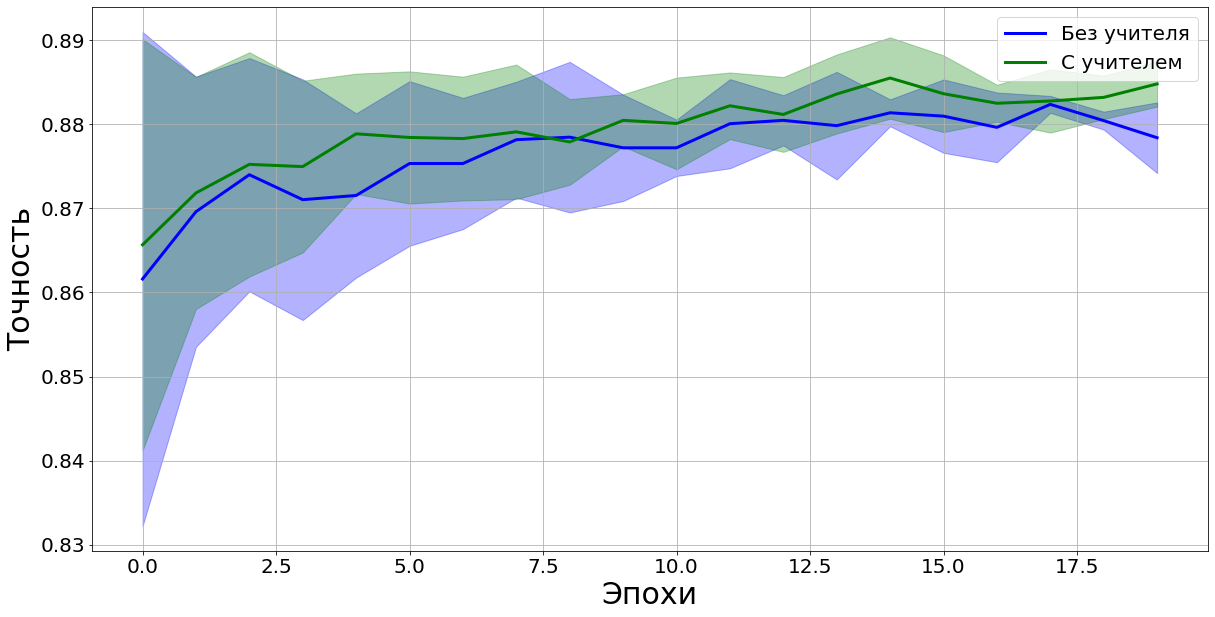
\includegraphics[width=0.5\textwidth]{results/acc}}
\subfloat[]
{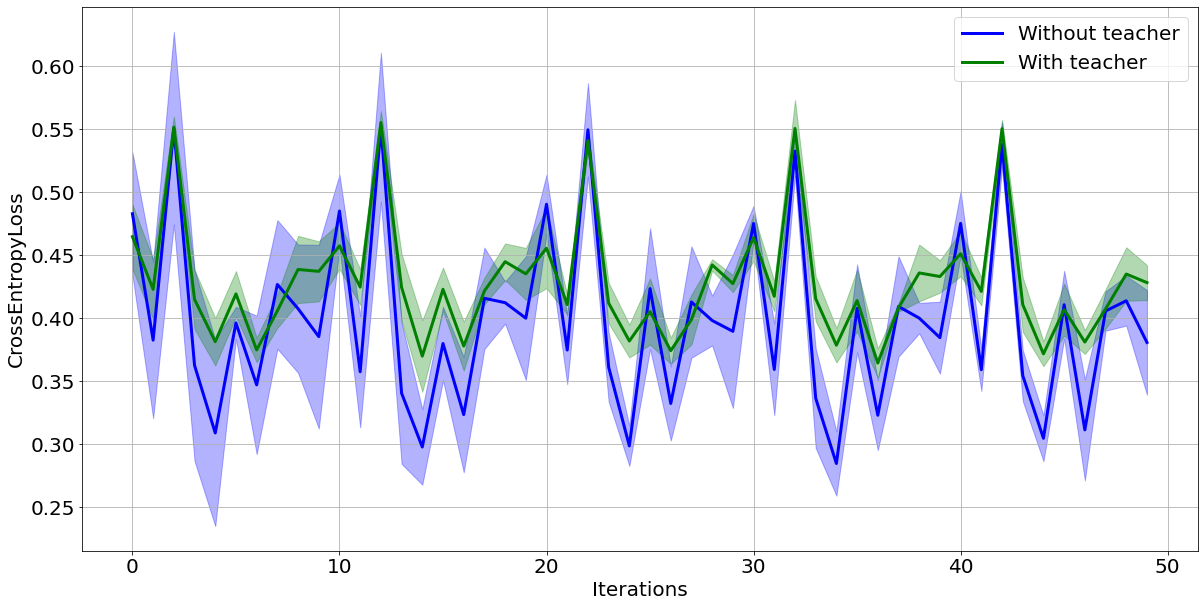
\includegraphics[width=0.5\textwidth]{results/loss}}\\
\caption{Качество аппроксимации на тестовой выборке. Все результаты усреднены по 5 запускам. a) точность; b) кросс-энтропийная ошибка между истинными и предсказанными учеником метками}
\end{figure}

На рис.1а показан график зависимости метрики точности на отложенной тестовой выборке между истинными метками объектов и метками предсказанными моделью ученика.

На рис.1б показан график зависимости кросс-энтропийной ошибки на отложенной тестовой выборке между истинными метками объектов и вероятностями, предсказанными моделью ученика.

На графиках видно, что модель, использующая метки учителя, показывает лучшее значение точности, при этом наблюдается значительное снижение кросс-энтропийной ошибки.


\begin{table}[h!t]
\begin{center}
\caption{Качество моделей}
\label{table_3}
\resizebox{\linewidth}{!}{
\begin{tabular}{|c|c|c|c|c|c|}
\hline
	Ученик & Учитель & Отображение $\varphi$ & Точность & \begin{tabular}[c]{@{}c@{}}Кросс-энтропийная\\ ошибка\end{tabular} & \begin{tabular}[c]{@{}c@{}}Интегральный\\ критерий\end{tabular}\\
	\hline
	\multicolumn{1}{|l|}{FashionMNIST-Train}
	& --- & --- & $0{,}878 \pm 0{,}004$ & $0{,}384 \pm 0{,}031$ & $7{,}151 \pm 0{,}459$ \\
	\hline
	\multicolumn{1}{|l|}{FashionMNIST-Train}
	& FashionMNIST-Train & --- & $\textbf{0{,}885} \pm \textbf{0{,}003}$ & $\textbf{0{,}329} \pm \textbf{0{,}002}$ & $\textbf{6{,}520} \pm \textbf{0{,}303}$ \\
\hline
\end{tabular}
}
\end{center}
\end{table}

В таблице~\ref{table_3} представлены результаты сравнения моделей ученика, полученных с использованием и без использования дистилляции.

\newpage
\paragraph{Обучение на малоресурсной части.}
Модель учителя обучается на многоресурсной части FashionMNIST-Big, а модель ученика обучается на малоресурсной части FashionMNIST-Small.

\begin{figure}[h!t]\center
\subfloat[]
{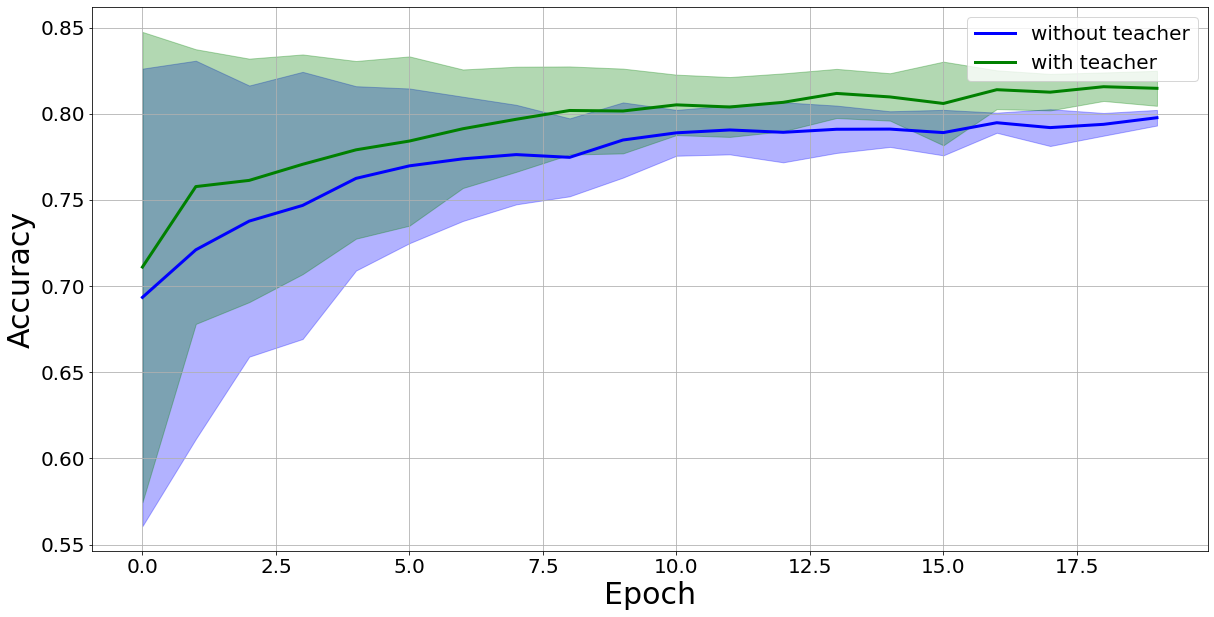
\includegraphics[width=0.5\textwidth]{results/small_acc}}
\subfloat[]
{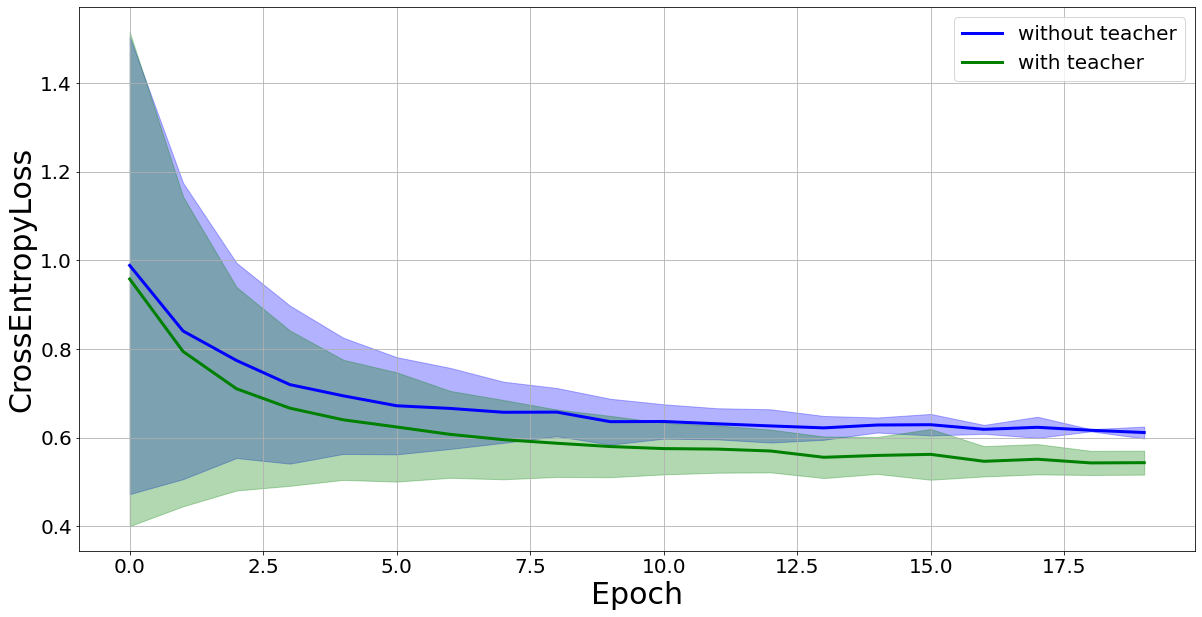
\includegraphics[width=0.5\textwidth]{results/small_loss}}\\
\caption{Качество аппроксимации на тестовой выборке. Все результаты усреднены по 5 запускам. a) точность; b) кросс-энтропийная ошибка между истинными и предсказанными учеником метками}
\end{figure}

На рис.2а показан график зависимости метрики точности на отложенной тестовой выборке между истинными метками объектов и метками, предсказанными моделью ученика.

На рис.2б показан график зависимости кросс-энтропийной ошибки на отложенной тестовой выборке между истинными метками объектов и вероятностями, предсказанными моделью ученика.

На графиках видно, что модель, использующая метки учителя, показывает лучшее значение точности, при этом наблюдается снижение кросс-энтропийной ошибки.

\begin{table}[h!t]
\begin{center}
\caption{Качество моделей}
\label{table_4}
\resizebox{\linewidth}{!}{
\begin{tabular}{|c|c|c|c|c|c|}
\hline
	Ученик & Учитель & Отображение $\varphi$ & Точность & \begin{tabular}[c]{@{}c@{}}Кросс-энтропийная \\ ошибка\end{tabular} & \begin{tabular}[c]{@{}c@{}}Интегральный\\ критерий\end{tabular}\\
	\hline
	\multicolumn{1}{|l|}{FashionMNIST-Train}
	& --- & --- & $0{,}878 \pm 0{,}004$ & $0{,}384 \pm 0{,}031$ & $7{,}151 \pm 0{,}459$ \\
	\hline
	\multicolumn{1}{|l|}{FashionMNIST-Train}
	& FashionMNIST-Train & --- & $\textbf{0{,}885} \pm \textbf{0{,}003}$ & $\textbf{0{,}329} \pm \textbf{0{,}002}$ & $\textbf{6{,}520} \pm \textbf{0{,}303}$ \\
	\hline \hline
	\multicolumn{1}{|l|}{FashionMNIST-Small}
	& --- & --- & $0{,}798 \pm 0{,}005$ & $0{,}666 \pm 0{,}065$ & $12{,}978 \pm 1{,}797$ \\
	\hline
	\multicolumn{1}{|l|}{FashionMNIST-Small}
	& FashionMNIST-Big & --- & $\textbf{0{,}813} \pm \textbf{0{,}007}$ & $\textbf{0{,}570} \pm \textbf{0{,}014}$ & $\textbf{11{,}484} \pm \textbf{1{,}607}$ \\
\hline
\end{tabular}
}
\end{center}
\end{table}

В таблице~\ref{table_4} представлены результаты сравнения моделей ученика, полученных с использованием и без использования дистилляции.

\newpage
\paragraph{Обучение на выборке с шумом.}
Добавим к многоресурсной части FashionMNIST-Big нормальный шум $\mathcal{N}\bigr(0,\frac{1}{10}\bigr)$ и обучим на нем модель учителя. Модель ученика обучается на малоресурсной части FashionMNIST-Small без шума.

\begin{figure}[h!t]\center
{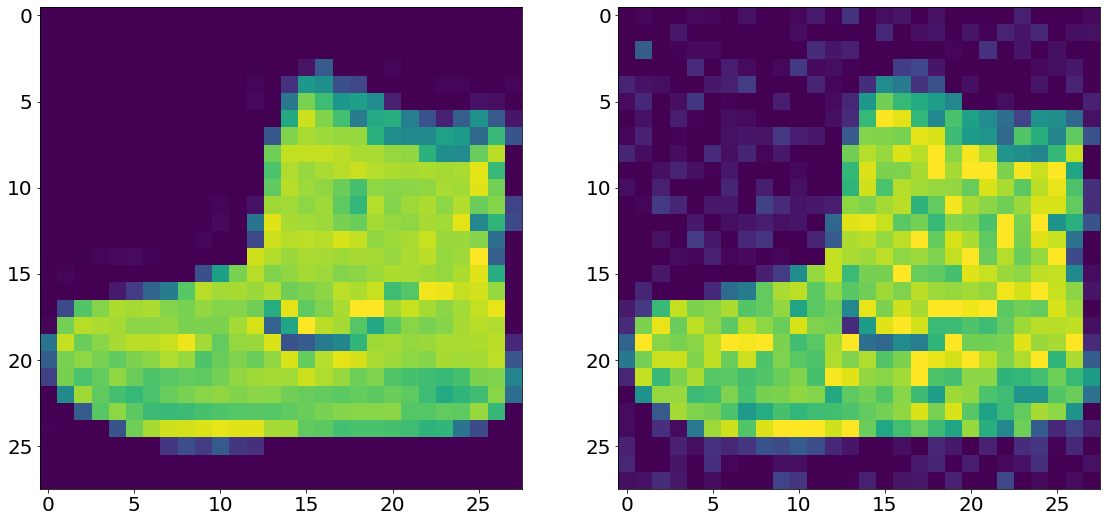
\includegraphics[width=0.5\textwidth]{results/noise}}
\caption{Сравнение объекта выборки до и после добавления шума}
\end{figure}

\begin{figure}[h!t]\center
\subfloat[]
{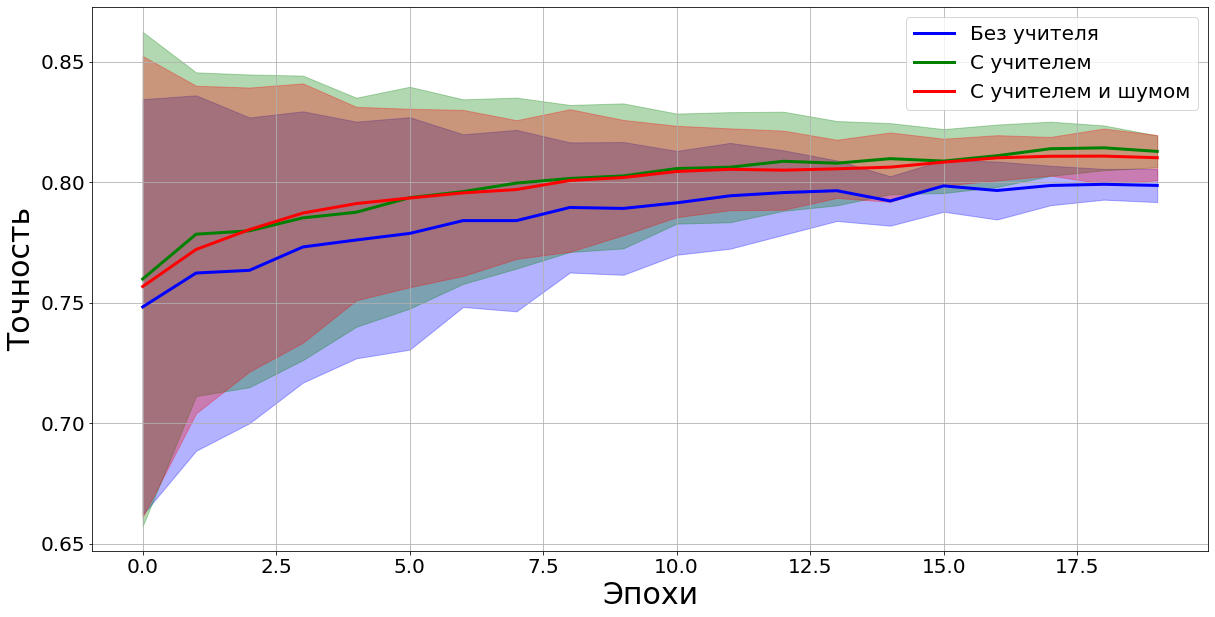
\includegraphics[width=0.5\textwidth]{results/noise_acc}}
\subfloat[]
{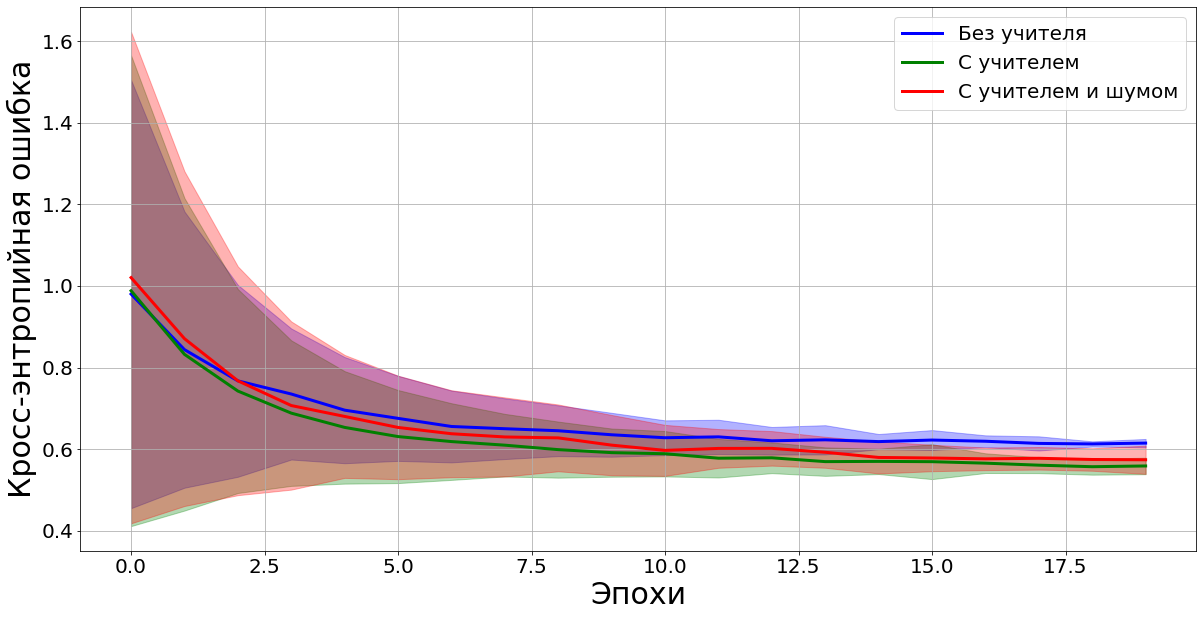
\includegraphics[width=0.5\textwidth]{results/noise_loss}}\\
\caption{Качество аппроксимации на тестовой выборке. Все результаты усреднены по 5 запускам. a) точность; b) кросс-энтропийная ошибка между истинными и предсказанными учеником метками}
\end{figure}

На рис.4а показан график зависимости метрики точности на отложенной тестовой выборке между истинными метками объектов и метками, предсказанными моделью ученика.

На рис.4б показан график зависимости кросс-энтропийной ошибки на отложенной тестовой выборке между истинными метками объектов и вероятностями, предсказанными моделью ученика.

На графиках видно, что значения точности и кросс-энтропийной ошибки модели, использующей метки учителя на выборке с шумом, лежат между соответствующими значениями для модели без учителя и для модели, использующей метки учителя на выборке без шума.

\begin{table}[h!t]
\begin{center}
\caption{Качество моделей}
\label{table_5}
\resizebox{\linewidth}{!}{
\begin{tabular}{|c|c|c|c|c|c|}
\hline
	Ученик & Учитель & Отображение $\varphi$ & Точность & \begin{tabular}[c]{@{}c@{}}Кросс-энтропийная\\ ошибка\end{tabular} & \begin{tabular}[c]{@{}c@{}}Интегральный\\ критерий\end{tabular}\\
	\hline
	\multicolumn{1}{|l|}{FashionMNIST-Train}
	& --- & --- & $0{,}878 \pm 0{,}004$ & $0{,}384 \pm 0{,}031$ & $7{,}151 \pm 0{,}459$ \\
	\hline
	\multicolumn{1}{|l|}{FashionMNIST-Train}
	& FashionMNIST-Train & --- & $\textbf{0{,}885} \pm \textbf{0{,}003}$ & $\textbf{0{,}329} \pm \textbf{0{,}002}$ & $\textbf{6{,}520} \pm \textbf{0{,}303}$ \\
	\hline \hline
	\multicolumn{1}{|l|}{FashionMNIST-Small}
	& --- & --- & $0{,}798 \pm 0{,}005$ & $0{,}666 \pm 0{,}065$ & $12{,}978 \pm 1{,}797$ \\
	\hline
	\multicolumn{1}{|l|}{FashionMNIST-Small}
	& FashionMNIST-Big & --- & $0{,}813 \pm 0{,}007$ & $0{,}570 \pm 0{,}014$ & $11{,}484 \pm 1{,}607$ \\
	\hline 
	\multicolumn{1}{|l|}{FashionMNIST-Small}
	& FashionMNIST-Big & Noise & $0{,}810 \pm 0{,}009$ & $0{,}565 \pm 0{,}024$ & $11{,}362 \pm 1{,}595$ \\
\hline
\end{tabular}
}
\end{center}
\end{table}

В таблице~\ref{table_5} представлены результаты сравнения моделей ученика, полученных с использованием и без использования дистилляции.

Получаем, что шум в выборке не влияет на качество.

\paragraph{Обучение на выборке с dilation.}
Применим к многоресурсной части FashionMNIST-Big сверточное преобразование с размером ядра, равным 5, и обучим на нем модель учителя. Модель ученика обучается на малоресурсной части FashionMNIST-Small.

\begin{figure}[h!t]\center
{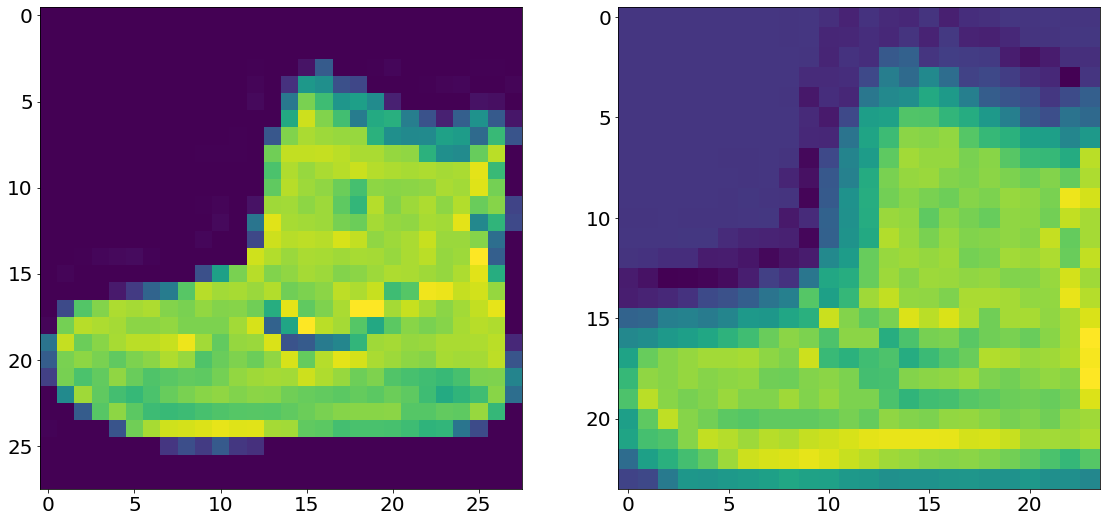
\includegraphics[width=0.5\textwidth]{results/dilation}}
\caption{Сравнение объекта выборки до и после преобразования}
\end{figure}

\begin{figure}[h!t]\center
\subfloat[]
{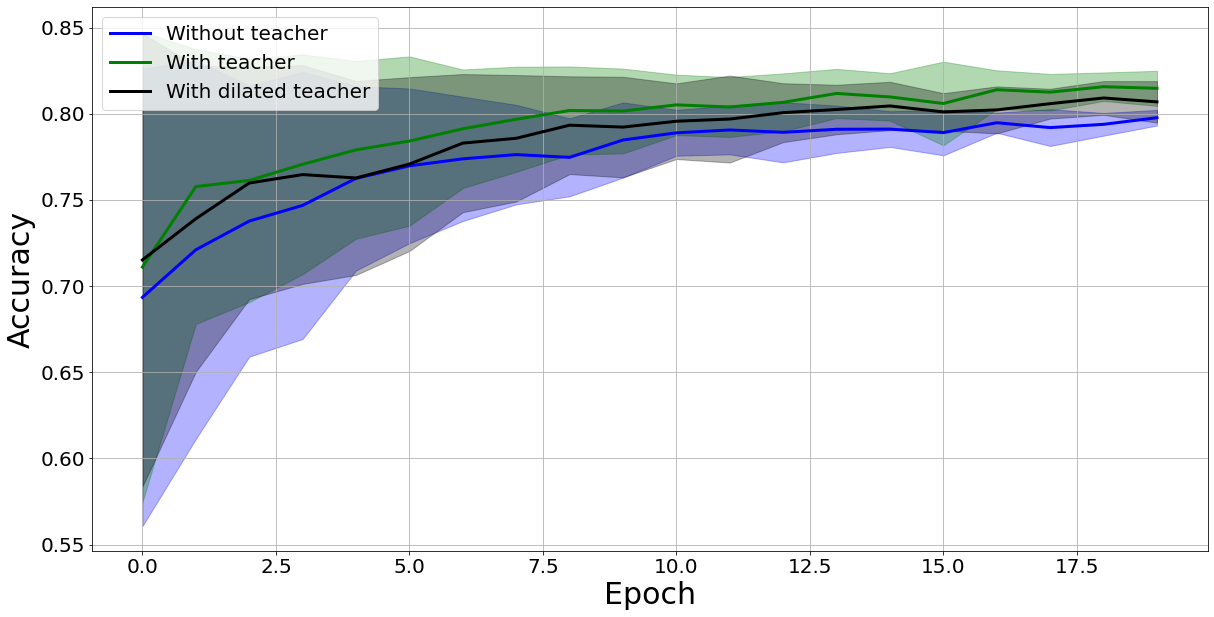
\includegraphics[width=0.5\textwidth]{results/dilation_acc}}
\subfloat[]
{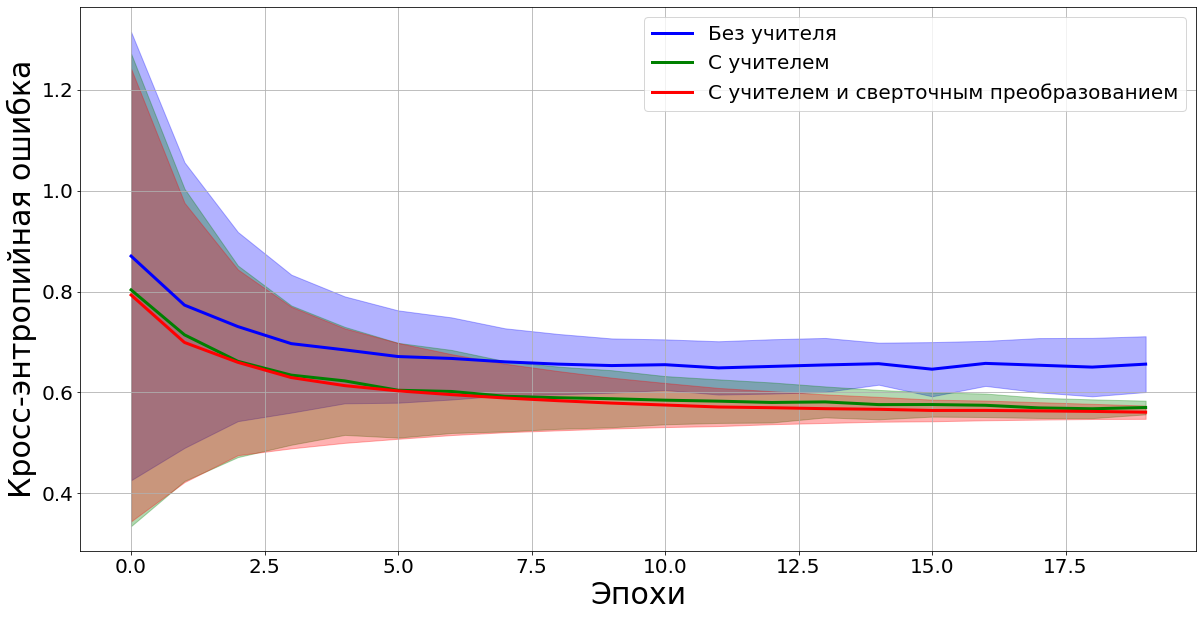
\includegraphics[width=0.5\textwidth]{results/dilation_loss}}\\
\caption{Качество аппроксимации на тестовой выборке. Все результаты усреднены по 5 запускам. a) точность; b) кросс-энтропийная ошибка между истинными и предсказанными учеником метками}
\end{figure}

На рис.6а показан график зависимости метрики точности на отложенной тестовой выборке между истинными метками объектов и метками, предсказанными моделью ученика.

На рис.6б показан график зависимости кросс-энтропийной ошибки на отложенной тестовой выборке между истинными метками объектов и вероятностями, предсказанными моделью ученика.

На графиках видно, что значения точности и кросс-энтропийной ошибки модели, использующей метки учителя на выборке с преобразованием, лежат между соответствующими значениями для модели без учителя и для модели, использующей метки учителя на выборке без преобразования.

\begin{table}[h!t]
\begin{center}
\caption{Качество моделей}
\label{table_6}
\resizebox{\linewidth}{!}{
\begin{tabular}{|c|c|c|c|c|c|}
\hline
	Ученик & Учитель & Отображение $\varphi$ & Точность & \begin{tabular}[c]{@{}c@{}}Кросс-энтропийная\\ ошибка\end{tabular} & \begin{tabular}[c]{@{}c@{}}Интегральный\\ критерий\end{tabular}\\
	\hline
	\multicolumn{1}{|l|}{FashionMNIST-Train}
	& --- & --- & $0{,}878 \pm 0{,}004$ & $0{,}384 \pm 0{,}031$ & $7{,}151 \pm 0{,}459$ \\
	\hline
	\multicolumn{1}{|l|}{FashionMNIST-Train}
	& FashionMNIST-Train & --- & $\textbf{0{,}885} \pm \textbf{0{,}003}$ & $\textbf{0{,}329} \pm \textbf{0{,}002}$ & $\textbf{6{,}520} \pm \textbf{0{,}303}$ \\
	\hline \hline
	\multicolumn{1}{|l|}{FashionMNIST-Small}
	& --- & --- & $0{,}798 \pm 0{,}005$ & $0{,}666 \pm 0{,}065$ & $12{,}978 \pm 1{,}797$ \\
	\hline
	\multicolumn{1}{|l|}{FashionMNIST-Small}
	& FashionMNIST-Big & --- & $0{,}813 \pm 0{,}007$ & $0{,}570 \pm 0{,}014$ & $11{,}484 \pm 1{,}607$ \\
	\hline 
	\multicolumn{1}{|l|}{FashionMNIST-Small}
	& FashionMNIST-Big & Noise & $0{,}810 \pm 0{,}009$ & $0{,}565 \pm 0{,}024$ & $11{,}362 \pm 1{,}595$ \\
	\hline
	\multicolumn{1}{|l|}{FashionMNIST-Small}
	& FashionMNIST-Big & Dilation & $\textbf{0{,}816} \pm \textbf{0{,}007}$ & $\textbf{0{,}561} \pm \textbf{0{,}013}$ & $\textbf{11{,}330} \pm \textbf{1{,}540}$ \\
\hline
\end{tabular}
}
\end{center}
\end{table}

В таблице~\ref{table_6} представлены результаты сравнения моделей ученика, полученных с использованием и без использования дистилляции.

\subsection{Вариационный автокодировщик}

В качестве преобразования элементов выборки FashionMNIST~\cite{FMNIST} в элементы выборки MNIST~\cite{MNIST} используем модель вариационного автокодировщика~\cite{VAE}, аппроксимирующую отображение $\varphi$.
\paragraph{Базовая модель автокодировщика.} Данная модель состоит из двух частей. Сначала строится вероятностное распределение в скрытом пространстве, которое позволяет генерировать скрытые представления для одного объекта. Далее с помощью декодировщика строится вероятностное распределение, позволяющее генерировать реконструкции исходного объекта.
\begin{enumerate}
    \item $q(\mathbf{z}|\mathbf{x}, \alpha)$ --- вероятностный кодировщик, где $\alpha$ --- параметры кодировщика;
    \item $p(\hat{\mathbf{x}}|\mathbf{z}, \beta)$ --- вероятностный декодировщик, где $\beta$ --- параметры декодировщика;
    \item функция потерь:
    \[
    \begin{aligned}
    \mathcal{L}_{\text{VAE}}(\alpha, \beta)=\sum\limits_{i=1}^{m}\mathsf{E}_{\mathbf{z}\sim q(\mathbf{z}|\mathbf{x}_{i}, \alpha)}\log{p(\mathbf{x}_{i}|\mathbf{z}, \beta)}-\mathsf{KL}(q(\mathbf{z}|\mathbf{x}_{i}, \alpha) || p(\mathbf{z})),
    \end{aligned}
    \]
    где
    $p(\mathbf{z})\sim \mathcal{N}(0,\sigma^{2}\mathbf{I})$ 
    --- априорное распределение.
\end{enumerate}
Получаем оптимизационную задачу:
$$\hat{\alpha}, \hat{\beta} = \arg\max_{\alpha, \beta} \mathcal{L}(\alpha, \beta).$$

\newpage
\paragraph{Генерация отображения из FashionMNIST в MNIST.}
Воспользуемся моделью вариационного автокодировщика~\cite{VAE} для преобразования изображений одежды из выборки FashionMNIST~\cite{FMNIST} в изображения цифр на основе выборки MNIST~\cite{MNIST}.

Сгенерируем синтетическую выборку, где каждому изображению одежды выборки FashionMNIST-Train будет соответстовать случайное изображение цифры из выборки MNIST-Train из того же класса.

\begin{figure}[h!t]\center
\subfloat[]
{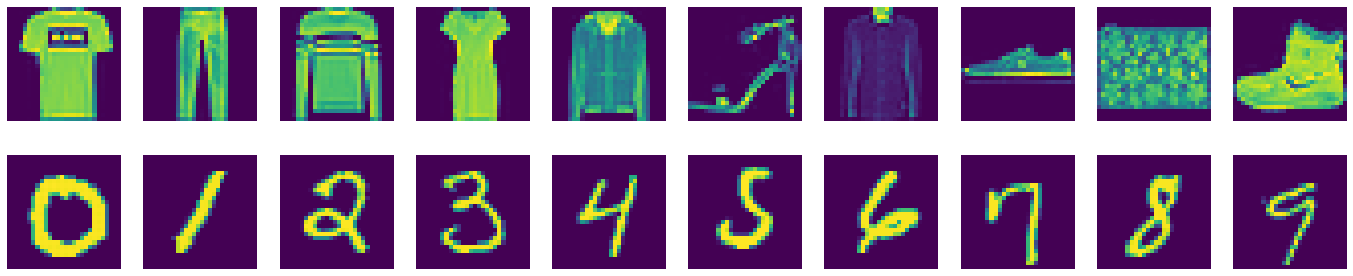
\includegraphics[width=0.8\textwidth]{results/fmnist_random_mnist_10.png}}
\qquad
\subfloat[]
{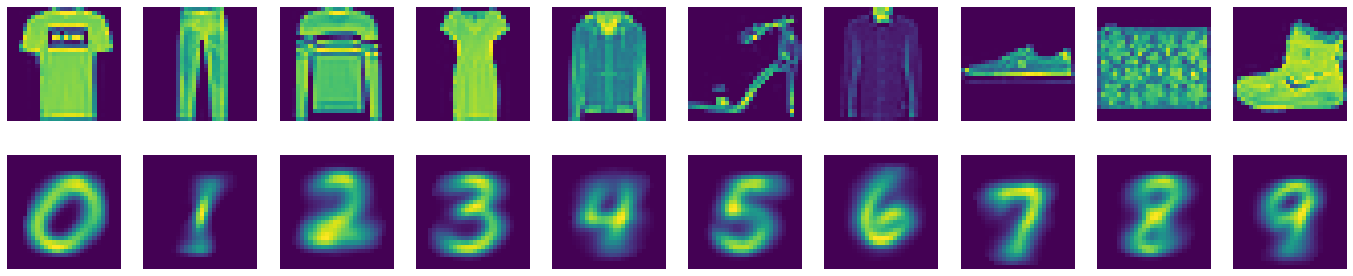
\includegraphics[width=0.8\textwidth]{results/fmnist_vae_mnist_10.png}}\\
\caption{a) Объекты синтетический выборки; b) Объекты исходной выборки до и после работы автокодировщика}
\end{figure}
Далее воспользуемся моделью вариационного автокодировщика, состоящего из одного кодировщика и двух декодировщиков, соответствующих генерации объектов цифр и одежды соответственно. Используем модель с размером скрытого представления, равным 64.

\begin{figure}[h!t]\center
{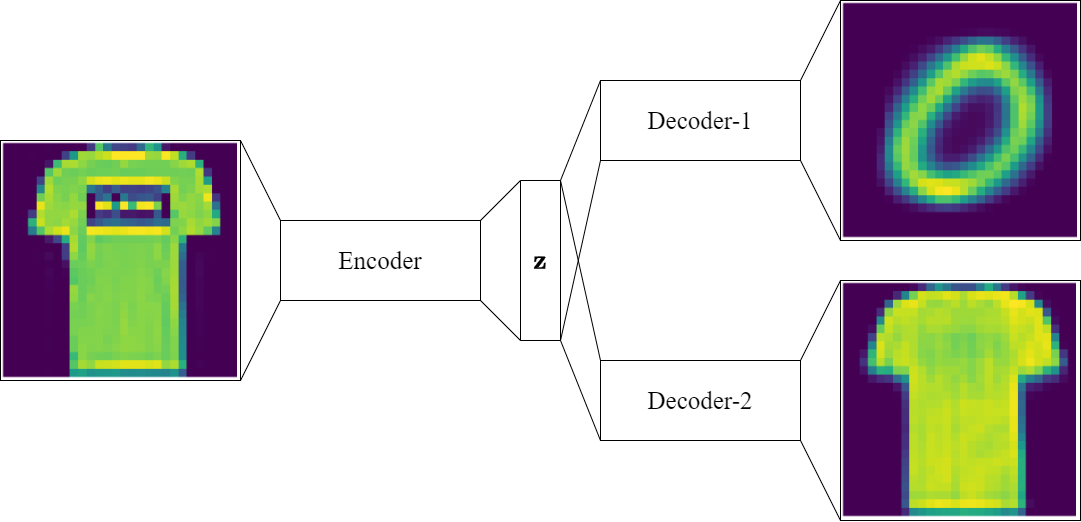
\includegraphics[width=0.8\textwidth]{results/VAE.png}}
\caption{Пример работы вариационного автокодировщика}
\end{figure}

На основе полученной выборки обучим модель вариационного автокодировщика, минимизируя ошибку между выходом модели и исходным значением --- изображением одежды и ошибку между выходом модели и целевым значением --- изображением цифр, соответствующего исходному объекту.

Полученная модель генеририрует семейство новых объектов --- изображений цифры и изображений одежды для одного и того же изображения одежды.

\newpage

Проанализируем изменение выхода модели при изменении случайного вектора в скрытом представлении. Для визуализации рассмотрим скрытое представление размерности 2:

\begin{figure}[h!t]\center
\subfloat[]
{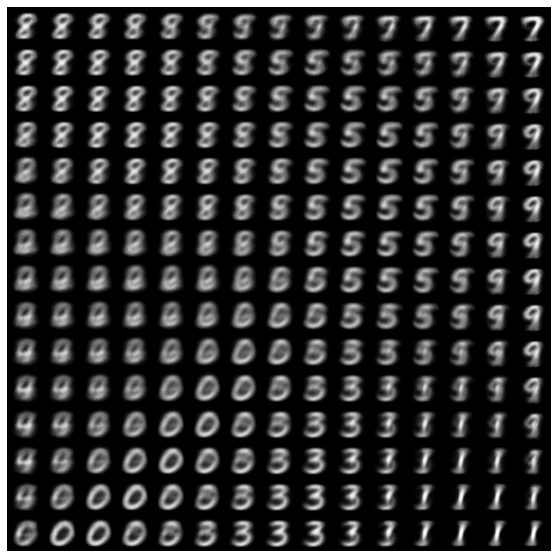
\includegraphics[width=0.4\textwidth]{results/decoder_digits.png}}
\qquad
\subfloat[]
{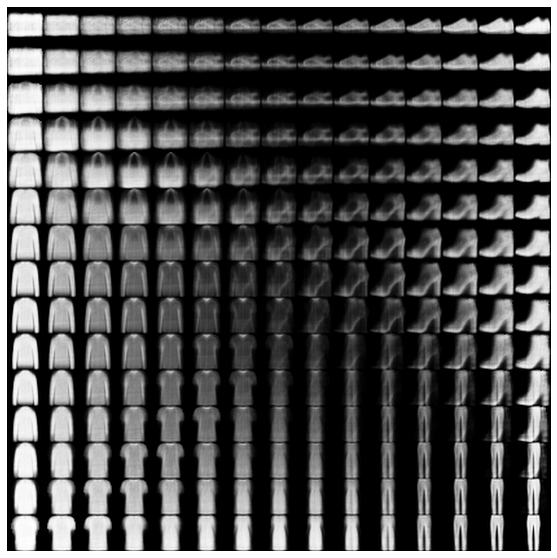
\includegraphics[width=0.4\textwidth]{results/decoder_fashion.png}}\\
\caption{Зависимость выхода модели от изменения вектора в скрытом представлении для генерации a) цифр; b) одежды}
\end{figure}

Видно, что при варьировании вектора в скрытом состоянии меняется также и выход автокодировщика. При этом всегда наблюдается равенство классов полученных цифр и предметов одежды, как представлено на рис.7а. То есть рис.9 не противоречит рис.7

Согласно определению 1.5 существует отображение из выборки FashionMNIST в выборку MNIST. Значит данные выборки являются близкими генеральными совокупностями и их можно использовать для задачи дистилляции для многодоменной выборки.

\subsection{Анализ качества модели, предложенной на\\
основе вариационного автокодировщика}

Модель учителя обучается на выборке MNIST-Big, а модель ученика на выборке FashionMNIST-Small. При этом обученная модель ученика использует метки учителя, на вход которого подается выход вариационного автокодировщика~\cite{VAE}, переводящего изображения одежды в изображения цифр.

Сравнивается качество аппроксимации без использования вариационного автокодировщика: модель ученика обучается на выборке FashionMNIST-Small, модель учителя обучается на выборке MNIST-Big и используется при обучении ученика, получая на вход изображения одежды без преобразования вариационным автокодировщиом.\\

\begin{figure}[h!t]\center
\subfloat[]
{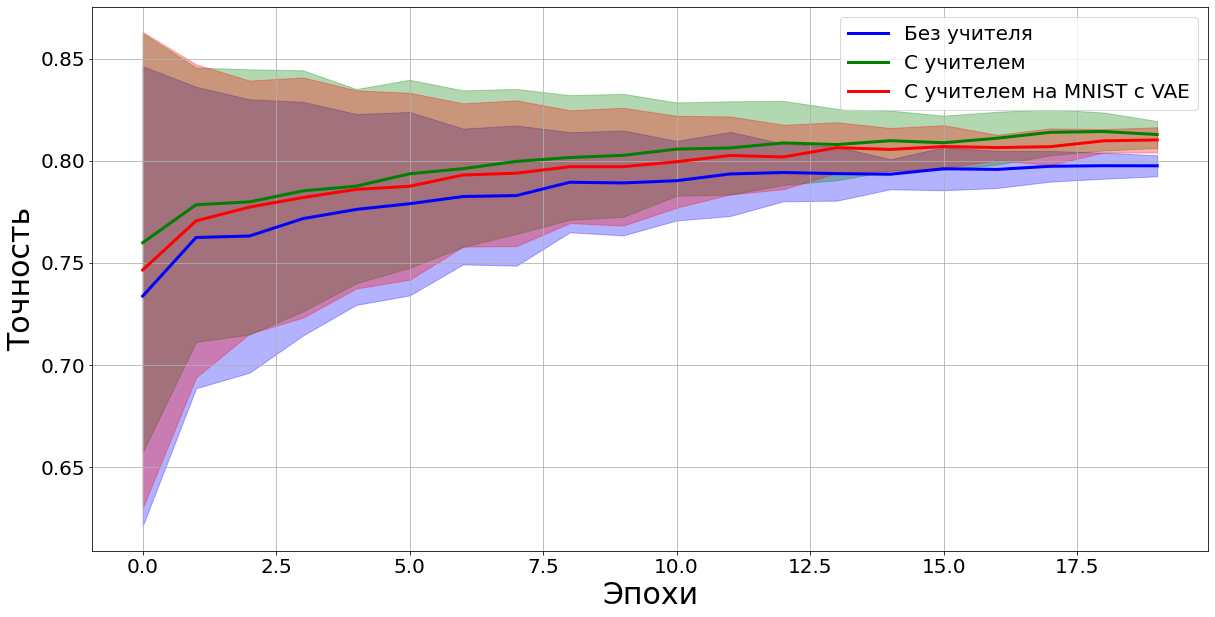
\includegraphics[width=0.5\textwidth]{results/vae_acc}}
\subfloat[]
{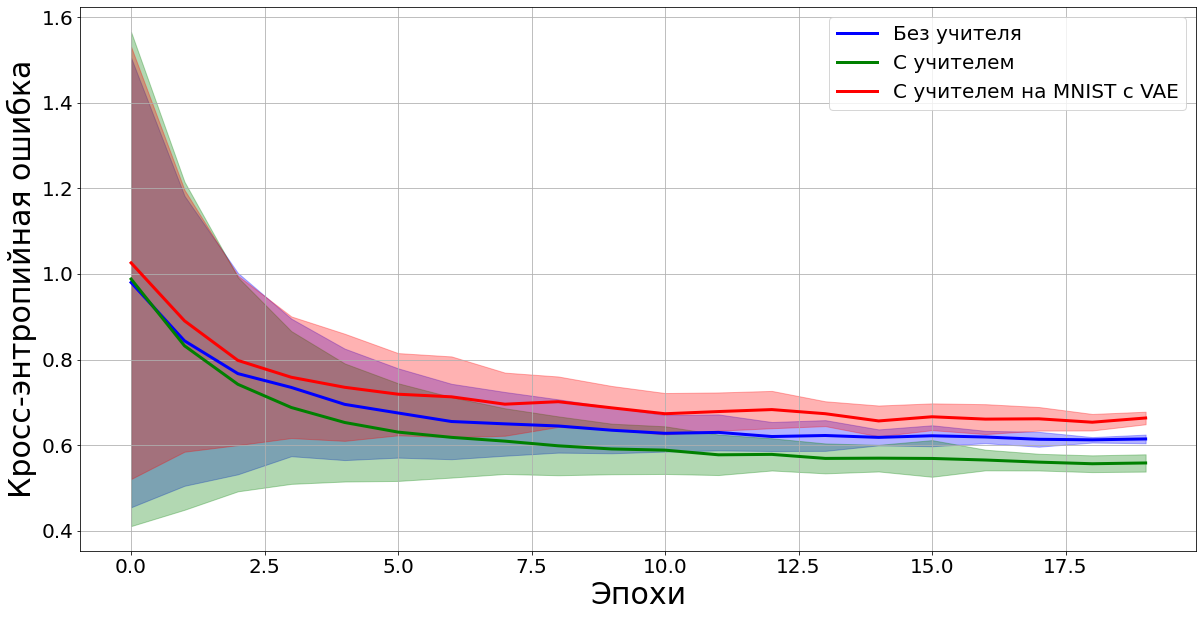
\includegraphics[width=0.5\textwidth]{results/vae_loss}}\\
\caption{Качество аппроксимации при использовании VAE на малодоменной выборке. Все результаты усреднены по 5 запускам. a) точность; b) кросс-энтропийная ошибка между истинными и предсказанными учеником метками}
\end{figure}

\begin{figure}[h!t]\center
\subfloat[]
{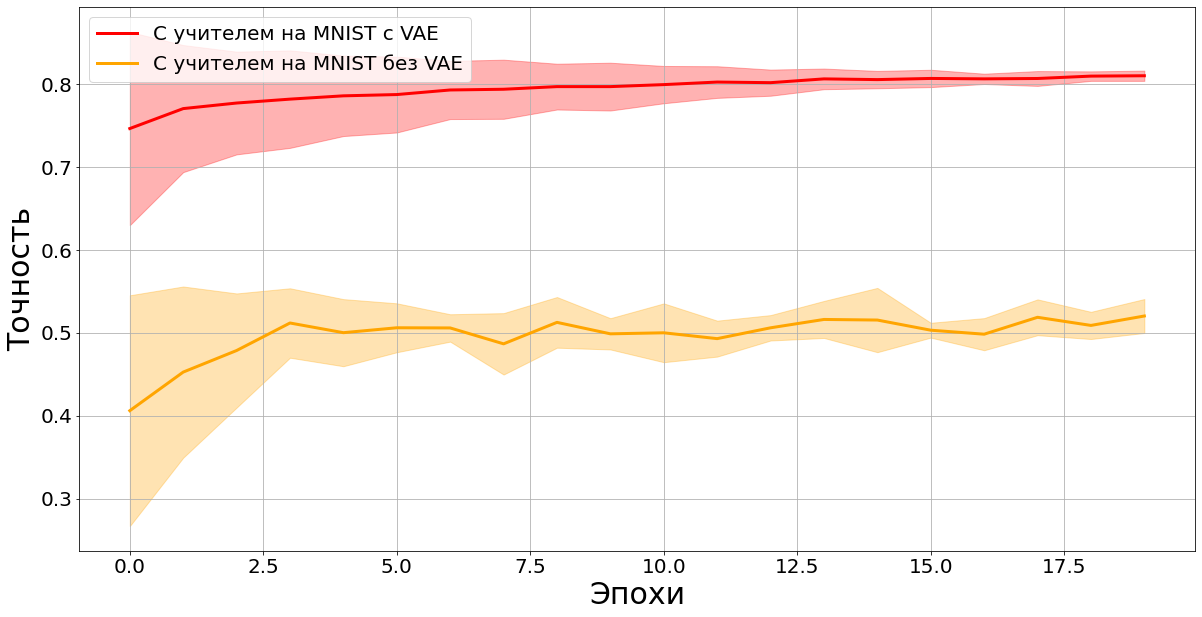
\includegraphics[width=0.5\textwidth]{results/vae_acc_comparison}}
\subfloat[]
{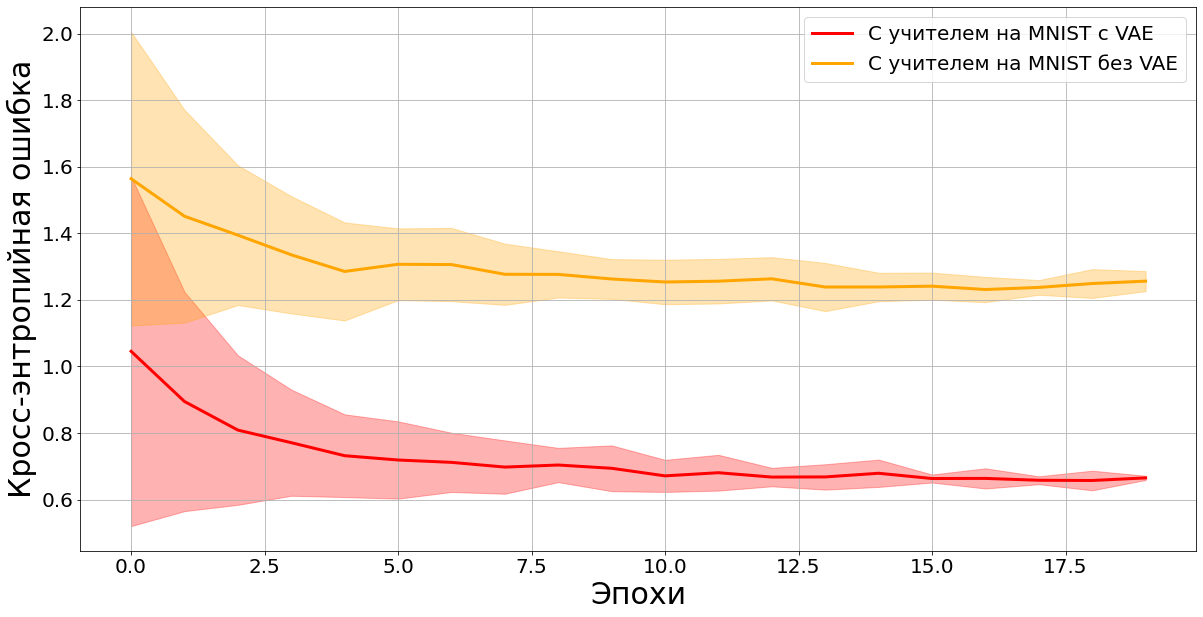
\includegraphics[width=0.5\textwidth]{results/vae_loss_comparison}}\\
\caption{Сравнение качества аппроксимации в зависимости от использования VAE на малодоменной выборке. Все результаты усреднены по 5 запускам. a) точность; b) кросс-энтропийная ошибка между истинными и предсказанными учеником метками}
\end{figure}

На графиках видно, что без использования отображения $\varphi$ модель становится более шумной с явным понижением качества аппроксимации.

\begin{table}[h!t]
\begin{center}
\caption{Качество моделей}
\label{table_7}
\resizebox{\linewidth}{!}{
\begin{tabular}{|c|c|c|c|c|c|}
\hline
	Ученик & Учитель & Отображение $\varphi$ & Точность & \begin{tabular}[c]{@{}c@{}}Кросс-энтропийная\\ ошибка\end{tabular} & \begin{tabular}[c]{@{}c@{}}Интегральный\\ критерий\end{tabular}\\
	\hline
	\multicolumn{1}{|l|}{FashionMNIST-Train}
	& --- & --- & $0{,}878 \pm 0{,}004$ & $0{,}384 \pm 0{,}031$ & $7{,}151 \pm 0{,}459$ \\
	\hline
	\multicolumn{1}{|l|}{FashionMNIST-Train}
	& FashionMNIST-Train & --- & $\textbf{0{,}885} \pm \textbf{0{,}003}$ & $\textbf{0{,}329} \pm \textbf{0{,}002}$ & $\textbf{6{,}520} \pm \textbf{0{,}303}$ \\
	\hline \hline
	\multicolumn{1}{|l|}{FashionMNIST-Small}
	& --- & --- & $0{,}798 \pm 0{,}005$ & $0{,}666 \pm 0{,}065$ & $12{,}978 \pm 1{,}797$ \\
	\hline
	\multicolumn{1}{|l|}{FashionMNIST-Small}
	& FashionMNIST-Big & --- & $0{,}813 \pm 0{,}007$ & $0{,}570 \pm 0{,}014$ & $11{,}484 \pm 1{,}607$ \\
	\hline 
	\multicolumn{1}{|l|}{FashionMNIST-Small}
	& FashionMNIST-Big & Noise & $0{,}810 \pm 0{,}009$ & $0{,}565 \pm 0{,}024$ & $11{,}362 \pm 1{,}595$ \\
	\hline
	\multicolumn{1}{|l|}{FashionMNIST-Small}
	& FashionMNIST-Big & Dilation & $\textbf{0{,}816} \pm \textbf{0{,}007}$ & $\textbf{0{,}561} \pm \textbf{0{,}013}$ & $\textbf{11{,}330} \pm \textbf{1{,}540}$ \\
	\hline \hline
	\multicolumn{1}{|l|}{FashionMNIST-Small}
	& MNIST-Big & VAE & $\textbf{0{,}810} \pm \textbf{0{,}006}$ & $\textbf{0{,}629} \pm \textbf{0{,}018}$ & $\textbf{12{,}657} \pm \textbf{1{,}455}$ \\
	\hline
	\multicolumn{1}{|l|}{FashionMNIST-Small}
	& MNIST-Big & --- & $0{,}520 \pm 0{,}020$ & $1{,}257 \pm 0{,}028$ & $24{,}642 \pm 1{,}462$ \\
\hline
\end{tabular}
}
\end{center}
\end{table}

В таблице~\ref{table_7} представлены результаты сравнения моделей ученика, полученных с использованием и без использования дистилляции.

\newpage
\subsection{Анализ качества модели на расширенной синтетически сгенерированной выборке}

На основе малоресурсной части выборки FashionMNIST-Small сформируем новую выборку, сгенерировав для каждого объекта одежды 70 изображений цифр с помощью модели вариационного автокодировщика~\cite{VAE}. Полученная выборка  состоит из обучающей и тестовой части, при этом обучающая часть разделяется на многоресурсную и малоресурсную части. Обучающая часть содержит 60000 объектов, многоресурсная часть содержит 59000 объектов, малоресурсная часть содержит 1000 объектов, а тестовая часть содержит 10000 объектов.

\begin{table}[h!t]
\begin{center}
\caption{Расширенная сгенерированная выборка}
\label{table_8}
\resizebox{\linewidth}{!}{
\begin{tabular}{|c|c|c|}
\hline
	Выборка & Пояснение &\ Размер выборки\\
	\hline
	\multicolumn{1}{|l|}{GeneratedMNIST-Train}
	& Обучающая часть& 60000\\
	\hline
	\multicolumn{1}{|l|}{GeneratedMNIST-Big}
	& Многоресурсная часть& 59000\\
	\hline
	\multicolumn{1}{|l|}{GeneratedMNIST-Small}
	& Малоресурсная часть& 1000\\
	\hline
	\multicolumn{1}{|l|}{GeneratedMNIST-Test}
	& Тестовая часть& 10000\\
\hline
\end{tabular}
}
\end{center}
\end{table}

Модель ученика обучается на малоресурсной части FashionMNIST-Small, модель учителя на многоресурсной части GeneratedMNIST-Big сгенерированной расширенной выборки и используется при обучении ученика.

\newpage

\begin{figure}[h!t]\center
\subfloat[]
{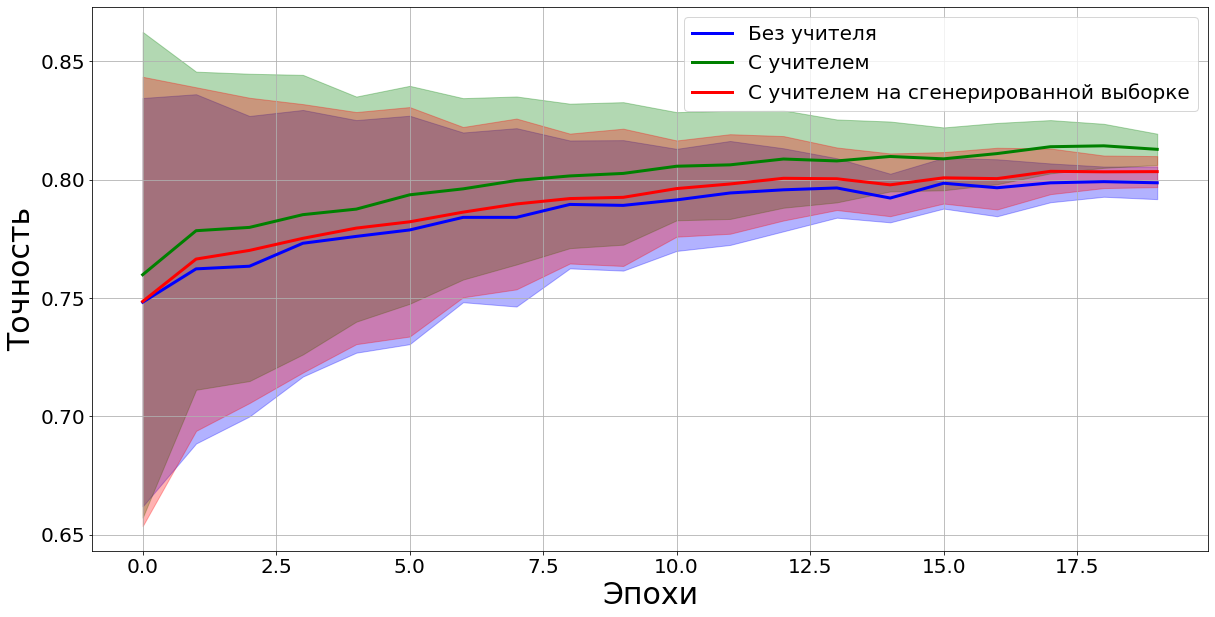
\includegraphics[width=0.5\textwidth]{results/ext_mnist_acc.png}}
\subfloat[]
{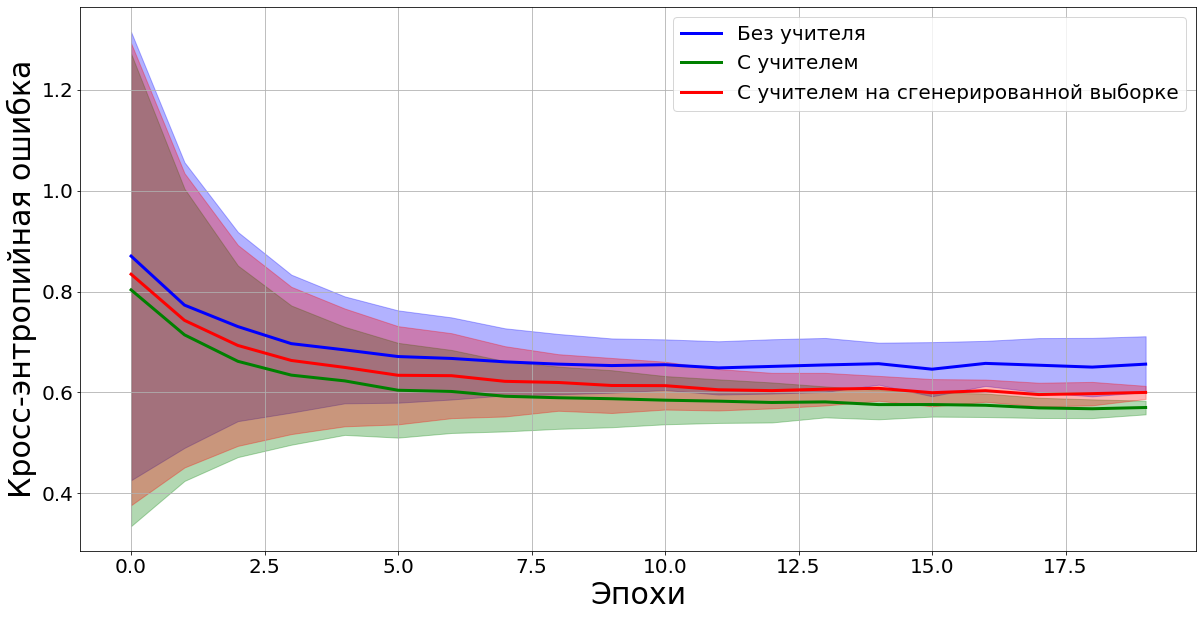
\includegraphics[width=0.5\textwidth]{results/ext_mnist_loss.png}}\\
\caption{Качество аппроксимации на тестовой выборке. Все результаты усреднены по 5 запускам. a) точность; b) кросс-энтропийная ошибка между истинными и предсказанными учеником метками}
\end{figure}

На графиках видно, что значения точности и кросс-энтропийной ошибки модели, использующей метки учителя, обученного на сгенерированной расширенной выборке, лежат между соответствующими значениями для модели без учителя и для модели, использующей метки учителя, обученного на многоресурсной части выборки.

\begin{table}[h!t]
\begin{center}
\caption{Качество моделей}
\label{table_9}
\resizebox{\linewidth}{!}{
\begin{tabular}{|c|c|c|c|c|c|}
\hline
	Ученик & Учитель & Отображение $\varphi$ & Точность & \begin{tabular}[c]{@{}c@{}}Кросс-энтропийная\\ ошибка\end{tabular} & \begin{tabular}[c]{@{}c@{}}Интегральный\\ критерий\end{tabular}\\
	\hline
	\multicolumn{1}{|l|}{FashionMNIST-Train}
	& --- & --- & $0{,}878 \pm 0{,}004$ & $0{,}384 \pm 0{,}031$ & $7{,}151 \pm 0{,}459$ \\
	\hline
	\multicolumn{1}{|l|}{FashionMNIST-Train}
	& FashionMNIST-Train & --- & $\textbf{0{,}885} \pm \textbf{0{,}003}$ & $\textbf{0{,}329} \pm \textbf{0{,}002}$ & $\textbf{6{,}520} \pm \textbf{0{,}303}$ \\
	\hline \hline
	\multicolumn{1}{|l|}{FashionMNIST-Small}
	& --- & --- & $0{,}798 \pm 0{,}005$ & $0{,}666 \pm 0{,}065$ & $12{,}978 \pm 1{,}797$ \\
	\hline
	\multicolumn{1}{|l|}{FashionMNIST-Small}
	& FashionMNIST-Big & --- & $0{,}813 \pm 0{,}007$ & $0{,}570 \pm 0{,}014$ & $11{,}484 \pm 1{,}607$ \\
	\hline 
	\multicolumn{1}{|l|}{FashionMNIST-Small}
	& FashionMNIST-Big & Noise & $0{,}810 \pm 0{,}009$ & $0{,}565 \pm 0{,}024$ & $11{,}362 \pm 1{,}595$ \\
	\hline
	\multicolumn{1}{|l|}{FashionMNIST-Small}
	& FashionMNIST-Big & Dilation & $\textbf{0{,}816} \pm \textbf{0{,}007}$ & $\textbf{0{,}561} \pm \textbf{0{,}013}$ & $\textbf{11{,}330} \pm \textbf{1{,}540}$ \\
	\hline \hline
	\multicolumn{1}{|l|}{FashionMNIST-Small}
	& MNIST-Big & VAE & $\textbf{0{,}810} \pm \textbf{0{,}006}$ & $\textbf{0{,}629} \pm \textbf{0{,}018}$ & $\textbf{12{,}657} \pm \textbf{1{,}455}$ \\
	\hline
	\multicolumn{1}{|l|}{FashionMNIST-Small}
	& MNIST-Big & --- & $0{,}520 \pm 0{,}020$ & $1{,}257 \pm 0{,}028$ & $24{,}642 \pm 1{,}462$ \\
	\hline \hline
	\multicolumn{1}{|l|}{FashionMNIST-Small}
	& GeneratedMNIST-Big & VAE & $0{,}803 \pm 0{,}007$ & $0{,}600 \pm 0{,}013$ & $12{,}019 \pm 1{,}629$ \\
\hline
\end{tabular}
}
\end{center}
\end{table}

В таблице~\ref{table_9} представлены результаты сравнения моделей ученика, полученных с использованием и без использования дистилляции.


\subsection{Анализ дистилляци на основе преобразования стиля изображений}
Используем подвыборку ImageNet --- набора изображений, для которого нужно решить задачу классификации на 10 классов. Выборка  состоит из обучающей и тестовой части, при этом обучающая часть разделяется на многоресурсную и малоресурсную части. Обучающая часть содержит 9469 объектов, многоресурсная часть содержит 8469  объектов, малоресурсная часть содержит 1000 объектов, а тестовая часть содержит 3925 объектов.

\begin{table}[h!t]
\begin{center}
\caption{Выборка ImageNet}
\label{table_10}
\begin{tabular}{|c|c|c|}
\hline
	Выборка & Пояснение &\ Размер выборки\\
	\hline
	\multicolumn{1}{|l|}{ImageNet-Train}
	& Обучающая часть& 9469\\
	\hline
	\multicolumn{1}{|l|}{ImageNet-Big}
	& Многоресурсная часть& 8469\\
	\hline
	\multicolumn{1}{|l|}{ImageNet-Small}
	& Малоресурсная часть& 1000\\
	\hline
	\multicolumn{1}{|l|}{ImageNet-Test}
	& Тестовая часть& 3925\\
\hline
\end{tabular}
\end{center}
\end{table}

В качестве модели учителя $\textbf{f}$ рассматривается нейронная сеть с пятью сверточными слоями и тремя полносвязными слоями, в качестве модели ученика рассматривается нейронная сеть с двумя сверточными слоями и двумя полносвязными слоями. Функция активации после каждого скрытого слоя --- ReLU.

\begin{table}[h!t]
\begin{center}
\caption{Структура учителя}
\label{table_11}
\resizebox{.8\linewidth}{!}{
\begin{tabular}{|c|c|c|}
\hline
	Слой & Размер входного вектора &\ Число параметров\\
	\hline
	\multicolumn{1}{|l|}{Входной слой}
	& (3, 200, 200) & 0 \\
	\hline
	\multicolumn{1}{|l|}{CONV1 (kernel size=5)}
	& (24, 196, 196) & 1800 \\
	\hline
	\multicolumn{1}{|l|}{POOL1}
	& (24, 98, 98) & 0 \\
	\hline
	\multicolumn{1}{|l|}{CONV2 (kernel size = 5)}
	& (48, 94, 94) & 28800 \\
	\hline
	\multicolumn{1}{|l|}{POOL2}
	& (48, 47, 47) & 0 \\
	\hline
	\multicolumn{1}{|l|}{CONV3 (kernel size = 8)}
	& (96, 40, 40) & 294912 \\
	\hline
	\multicolumn{1}{|l|}{POOL3}
	& (96, 20, 20) & 0 \\
	\hline
    \multicolumn{1}{|l|}{CONV4 (kernel size = 5)}
	& (192, 16, 16) & 460800 \\
	\hline
	\multicolumn{1}{|l|}{POOL4}
	& (192, 8, 8) & 0 \\
    \hline
	\multicolumn{1}{|l|}{CONV5 (kernel size = 7)}
	& (384, 2, 2) & 3612672 \\
	\hline
	\multicolumn{1}{|l|}{POOL5}
	& (384, 1, 1) & 0 \\
	\hline
	\multicolumn{1}{|l|}{Полносвязный слой}
	& (384) & 0 \\
	\hline
	\multicolumn{1}{|l|}{Полносвязный слой}
	& (120) & 46080 \\
	\hline
	\multicolumn{1}{|l|}{Полносвязный слой}
	& (84) & 10080 \\
	\hline
	\multicolumn{1}{|l|}{Полносвязный слой}
	& (10) & 840 \\
	\hline
	\multicolumn{1}{|l|}{}
	& & $\sum=4455984$ \\
\hline
\end{tabular}
}
\end{center}
\end{table}

\begin{table}[h!t]
\begin{center}
\caption{Структура ученика}
\label{table_12}
\resizebox{.8\linewidth}{!}{
\begin{tabular}{|c|c|c|}
\hline
	Слой & Размер входного вектора &\ Число параметров\\
	\hline
	\multicolumn{1}{|l|}{Входной слой}
	& (3, 200, 200) & 0 \\
	\hline
	\multicolumn{1}{|l|}{CONV1 (kernel size=5)}
	& (24, 196, 196) & 1800 \\
	\hline
	\multicolumn{1}{|l|}{POOL1}
	& (24, 98, 98) & 0 \\
	\hline
	\multicolumn{1}{|l|}{CONV2 (kernel size = 5)}
	& (48, 94, 94) & 28800 \\
	\hline
	\multicolumn{1}{|l|}{POOL2}
	& (48, 47, 47) & 0 \\
	\hline
	\multicolumn{1}{|l|}{Полносвязный слой}
	& (106032) & 0 \\
	\hline
	\multicolumn{1}{|l|}{Полносвязный слой}
	& (120) & 12723840 \\
	\hline
	\multicolumn{1}{|l|}{Полносвязный слой}
	& (10) & 1200 \\
	\hline
	\multicolumn{1}{|l|}{}
	& & $\sum=12755640$ \\
\hline
\end{tabular}
}
\end{center}
\end{table}

Применим к многоресурсной части ImageNet-Big преобразование стиля на основе сверточной нейронной сети VGG-19 и обучим на ней модель учителя. Модель ученика обучается на малоресурсной части ImageNet-Small без преобразования.

\begin{figure}[h!t]\center
{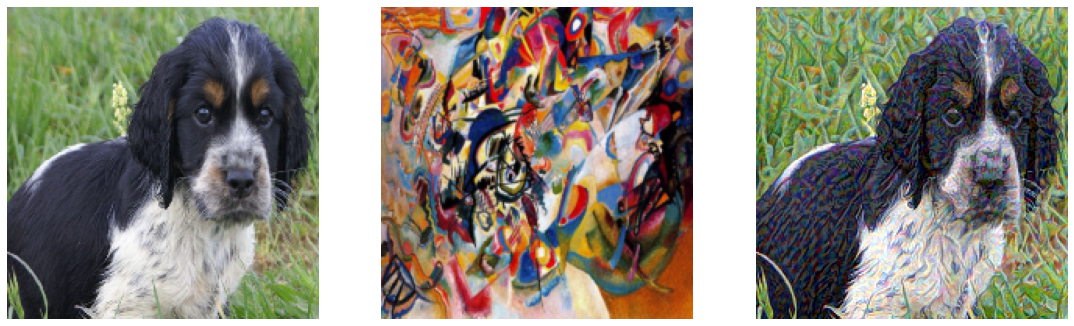
\includegraphics[width=1.0 \textwidth]{results/styletransfer.png}}
\caption{Сравнение объекта выборки до и после преобразования}
\end{figure}

\begin{figure}[h!t]\center
\subfloat[]
{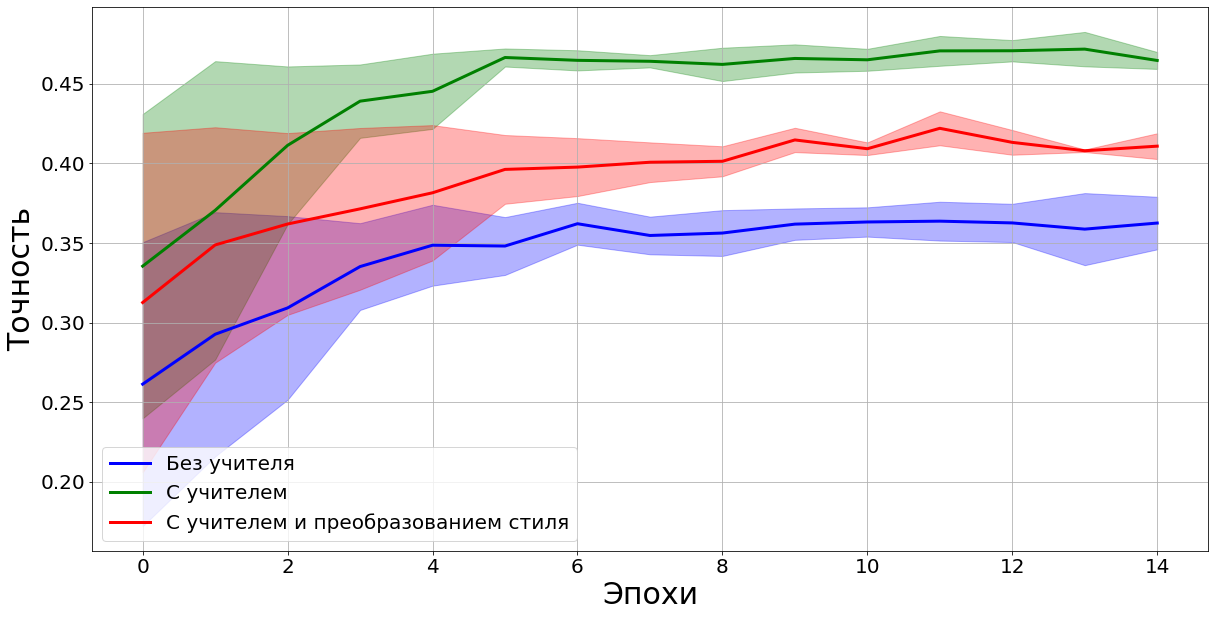
\includegraphics[width=0.5\textwidth]{results/styletransfer_acc.png}}
\subfloat[]
{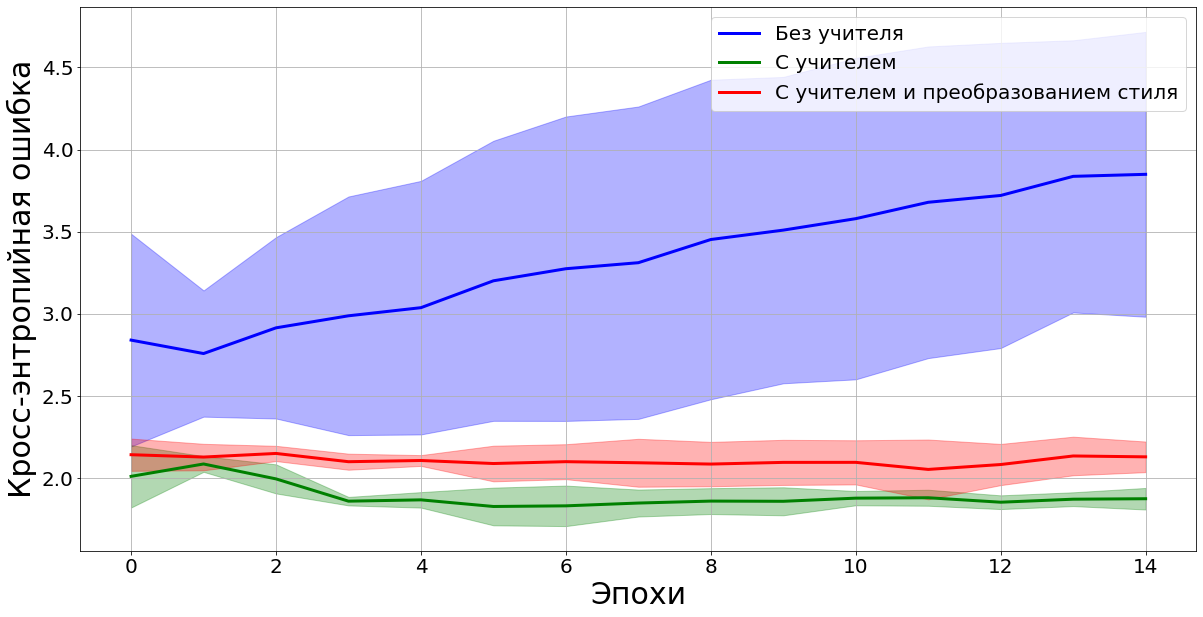
\includegraphics[width=0.5\textwidth]{results/styletransfer_loss.png}}\\
\caption{Качество аппроксимации на тестовой выборке. Все результаты усреднены по 3 запускам. a) точность; b) кросс-энтропийная ошибка между истинными и предсказанными учеником метками}
\end{figure}

На рис.14а показан график зависимости метрики точности на отложенной тестовой выборке между истинными метками объектов и метками, предсказанными моделью ученика.

На рис.14б показан график зависимости кросс-энтропийной ошибки на отложенной тестовой выборке между истинными метками объектов и вероятностями, предсказанными моделью ученика.

На графиках видно, что значения точности и кросс-энтропийной ошибки модели, использующей метки учителя на выборке с преобразованием, лежат между соответствующими значениями для модели без учителя и для модели, использующей метки учителя на выборке без преобразования.

\newpage
\begin{table}[h!t]
\begin{center}
\caption{Качество моделей}
\label{table_13}
\resizebox{\linewidth}{!}{
\begin{tabular}{|c|c|c|c|c|c|}
\hline
	Ученик & Учитель & Отображение $\varphi$ & Точность & \begin{tabular}[c]{@{}c@{}}Кросс-энтропийная\\ ошибка\end{tabular} & \begin{tabular}[c]{@{}c@{}}Интегральный\\ критерий\end{tabular}\\
	\hline
	\multicolumn{1}{|l|}{ImageNet-Small}
	& --- & --- & $0{,}363 \pm 0{,}017$ & $3{,}849 \pm 0{,}866$ & $46{,}615 \pm 11{,}498$ \\
    \hline
	\multicolumn{1}{|l|}{ImageNet-Small}
	& ImageNet-Big & --- & $\textbf{0{,}465} \pm \textbf{0{,}005}$ & $\textbf{1{,}876} \pm \textbf{0{,}066}$ & $\textbf{26{,}488} \pm \textbf{0{,}996}$ \\
    \hline
	\multicolumn{1}{|l|}{ImageNet-Small}
	& ImageNet-Big & StyleTransfer & $0{,}411 \pm 0{,}008$ & $2{,}131 \pm 0{,}093$ & $29{,}476 \pm 1{,}495$ \\
\hline
\end{tabular}
}
\end{center}
\end{table}

В таблице~\ref{table_13} представлены результаты сравнения моделей ученика, полученных с использованием и без использования дистилляции.

\newpage
\subsection{Анализ дистилляции для задачи регрессии}
Сгенерируем синтетическую выборку из нормального распределения и разделим ее на обучающую и тестовую часть. При этом обучающая часть разделяется на многоресурсную и малоресурсную части. Обучающая часть содержит 9000 объектов, многоресурсная часть содежит 8700 объектов, малоресурсная часть содержит 300 объектов, а тестовая часть содержит 1000 объектов.

\begin{table}[h!t]
\begin{center}
\caption{Выборки}
\label{table_14}
\begin{tabular}{|c|c|c|}
\hline
	Выборка & Пояснение &\ Размер выборки\\
	\hline
	\multicolumn{1}{|l|}{Reg-Train}
	& Обучающая часть& 9000\\
	\hline
	\multicolumn{1}{|l|}{Reg-Big}
	& Многоресурсная часть& 8700\\
	\hline
	\multicolumn{1}{|l|}{Reg-Small}
	& Малоресурсная часть& 300\\
	\hline
	\multicolumn{1}{|l|}{Reg-Test}
	& Тестовая часть& 1000\\
\hline
\end{tabular}
\end{center}
\end{table}

В качестве модели учителя $\textbf{f}$ и модели ученика $\textbf{g}$ рассматривается многослойный перцептрон с четырьми и одним скрытыми слоями соответственно:

\begin{table}[h!t]
\begin{center}
\caption{Описание моделей}
\label{table_15}
\begin{tabular}{|c|c|c|}
\hline
	 & Учитель &\ Ученик\\
	\hline
	\multicolumn{1}{|l|}{Структура}
	& [100,256,128,64,64,1]& [100,32,1]\\
	\hline
	\multicolumn{1}{|l|}{Число параметров}
	& 70720 & 3232\\
\hline

\end{tabular}
\end{center}
\end{table}

Функция активации после каждого скрытого слоя --- ReLu.

\paragraph{Обучение на всей выборке.}
Модели учителя и ученика обучаются на обучающей части Reg-Train.

\begin{figure}[h!t]\center
{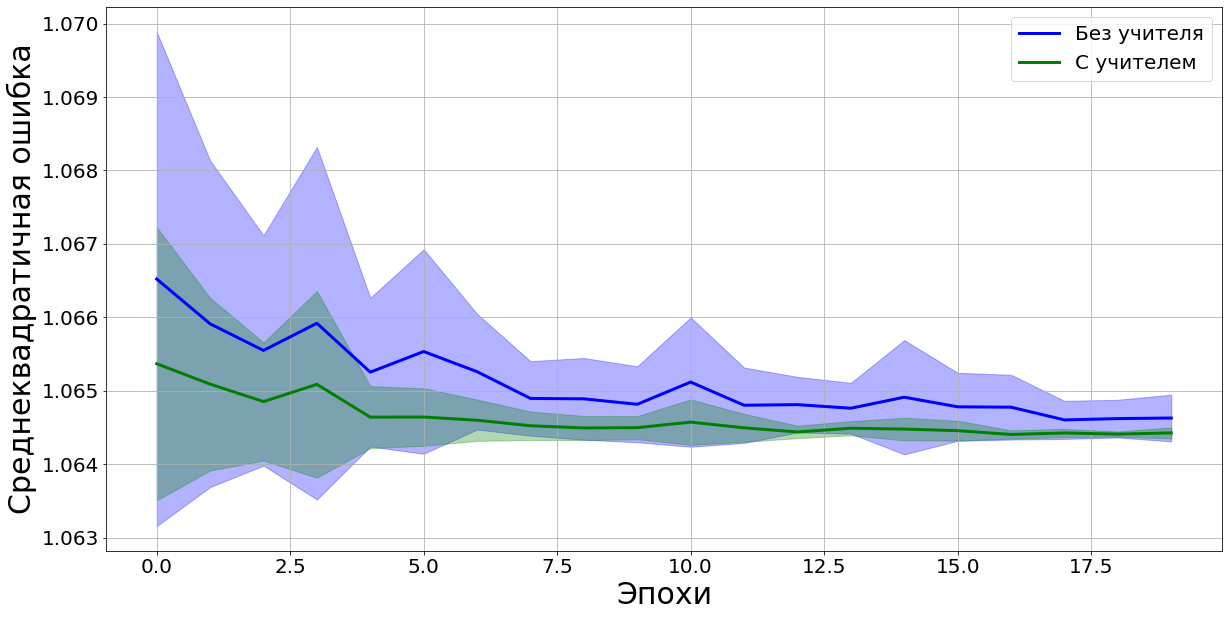
\includegraphics[width=0.8\textwidth]{results/reg_loss}}\\
\caption{Среднеквадратичная ошибка между истинными и предсказанными учеником значениями на тестовой выборке. Все результаты усреднены по 5 запускам.}
\end{figure}

На рис.13 показан график зависимости среднеквадратичной ошибки на отложенной тестовой выборке между истинными значениями объектов и значениями, предсказанными моделью ученика.

На графике видно, что модель, использующая ответы учителя, показывает лучшее значение среднеквадратичной ошибки.

\begin{table}[h!t]
\begin{center}
\caption{Качество моделей}
\label{table_16}
\resizebox{\linewidth}{!}{
\begin{tabular}{|c|c|c|c|c|c|}
\hline
	Ученик & Учитель & Отображение $\varphi$ & Точность & \begin{tabular}[c]{@{}c@{}}Среднеквадратичная\\ ошибка\end{tabular} & \begin{tabular}[c]{@{}c@{}}Интегральный\\ критерий\end{tabular}\\
\hline
	\multicolumn{1}{|l|}{Reg-Train}
	& --- & --- & --- & $1{,}0646 \pm 0{,}0003$ & --- \\
    \hline
	\multicolumn{1}{|l|}{Reg-Train}
	& Reg-Train & --- & --- & $\textbf{1{,}0644} \pm \textbf{0{,}0001}$ & --- \\
\hline
\end{tabular}
}
\end{center}
\end{table}

В таблице~\ref{table_16} представлены результаты сравнения моделей ученика, полученных с использованием и без использования дистилляции.

\paragraph{Обучение на малоресурсной части.}
Модель учителя обучается на многоресурсной части Reg-Big, а модель ученика обучается на малоресурсной части Reg-Small.

\begin{figure}[h!t]\center
{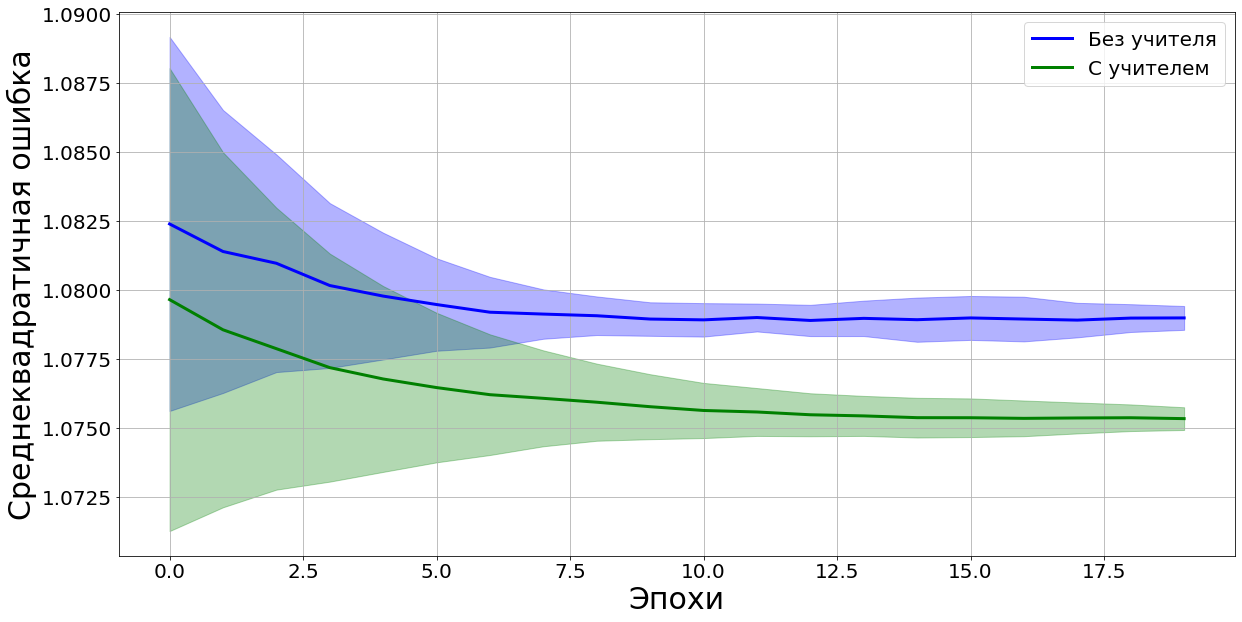
\includegraphics[width=0.8\textwidth]{results/reg_small_loss}}\\
\caption{Среднеквадратичная ошибка между истинными и предсказанными учеником значениями на тестовой выборке. Все результаты усреднены по 5 запускам.}
\end{figure}

На рис.16 показан график зависимости среднеквадратичной ошибки на отложенной тестовой выборке между истинными значениями объектов и значениями, предсказанными моделью ученика.

На графике видно, что модель, использующая ответы учителя, показывает лучшее значение среднеквадратичной ошибки.

\begin{table}[h!t]
\begin{center}
\caption{Качество моделей}
\label{table_17}
\resizebox{\linewidth}{!}{
\begin{tabular}{|c|c|c|c|c|c|}
\hline
	Ученик & Учитель & Отображение $\varphi$ & Точность & \begin{tabular}[c]{@{}c@{}}Среднеквадратичная\\ ошибка\end{tabular} & \begin{tabular}[c]{@{}c@{}}Интегральный\\ критерий\end{tabular}\\
	\hline
	\multicolumn{1}{|l|}{Reg-Train}
	& --- & --- & --- & $1{,}0646 \pm 0{,}0003$ & --- \\
    \hline
	\multicolumn{1}{|l|}{Reg-Train}
	& Reg-Train & --- & --- & $\textbf{1{,}0644} \pm \textbf{0{,}0001}$ & --- \\
	\hline \hline
	\multicolumn{1}{|l|}{Reg-Small}
	& --- & --- & --- & $1{,}0790 \pm 0{,}0004$ & --- \\
    \hline
	\multicolumn{1}{|l|}{Reg-Small}
	& Reg-Big & --- & --- & $\textbf{1{,}0753} \pm \textbf{0{,}0004}$ & --- \\
\hline
\end{tabular}
}
\end{center}
\end{table}

В таблице~\ref{table_17} представлены результаты сравнения моделей ученика, полученных с использованием и без использования дистилляции.

\paragraph{Обучение на выборке с преобразованием}
Добавим к многоресурсной части Reg-Big преобразование $\sin{x}$ и обучим на ней модель учителя. Модель ученика обучается на малоресурсной части Reg-Small без преобразования.

\begin{figure}[h!t]\center
{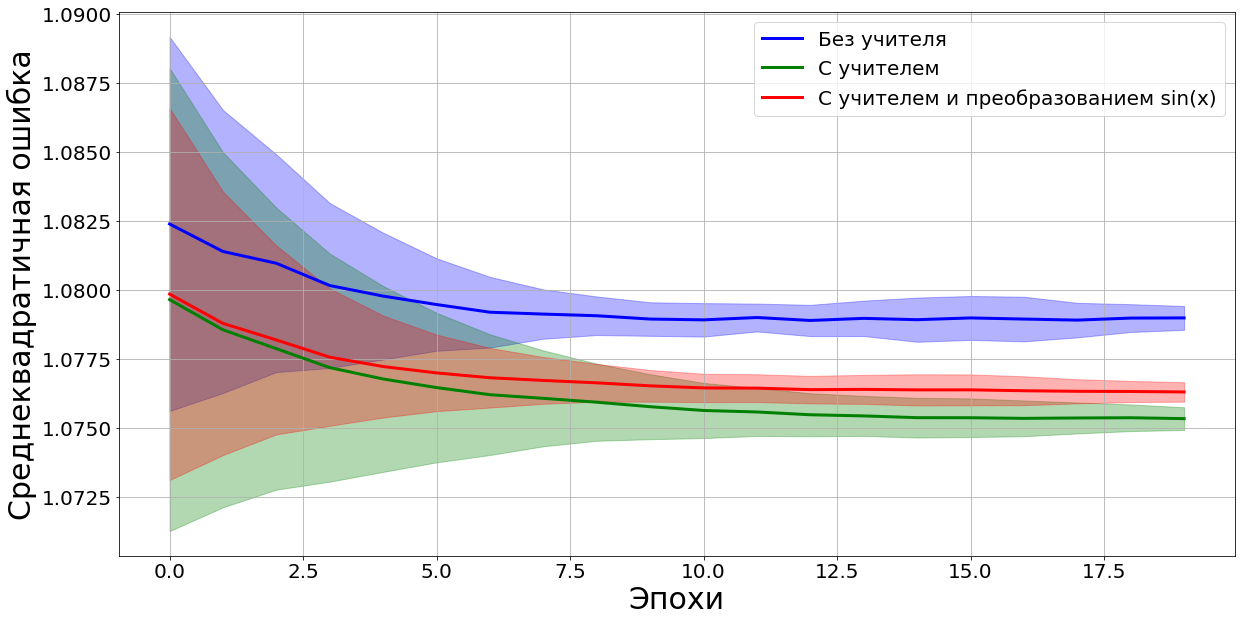
\includegraphics[width=0.8\textwidth]{results/reg_sin_loss}}\\
\caption{Среднеквадратичная ошибка между истинными и предсказанными учеником значениями на тестовой выборке. Все результаты усреднены по 5 запускам.}
\end{figure}

На рис.17 показан график зависимости среднеквадратичной ошибки на отложенной тестовой выборке между истинными значениями объектов и значениями, предсказанными моделью ученика.

На графике видно, что модель, использующая ответы учителя, показывает лучшее значение среднеквадратичной ошибки.

\begin{table}[h!t]
\begin{center}
\caption{Качество моделей}
\label{table_18}
\resizebox{\linewidth}{!}{
\begin{tabular}{|c|c|c|c|c|c|}
\hline
	Ученик & Учитель & Отображение $\varphi$ & Точность & \begin{tabular}[c]{@{}c@{}}Среднеквадратичная \\ ошибка\end{tabular} & \begin{tabular}[c]{@{}c@{}}Интегральный\\ критерий\end{tabular}\\
	\hline
	\multicolumn{1}{|l|}{Reg-Train}
	& --- & --- & --- & $1{,}0646 \pm 0{,}0003$ & --- \\
    \hline
	\multicolumn{1}{|l|}{Reg-Train}
	& Reg-Train & --- & --- & $\textbf{1{,}0644} \pm \textbf{0{,}0001}$ & --- \\
	\hline \hline
	\multicolumn{1}{|l|}{Reg-Small}
	& --- & --- & --- & $1{,}0790 \pm 0{,}0004$ & --- \\
    \hline
	\multicolumn{1}{|l|}{Reg-Small}
	& Reg-Big & --- & --- & $\textbf{1{,}0753} \pm \textbf{0{,}0004}$ & --- \\
    \hline
	\multicolumn{1}{|l|}{Reg-Small}
	& Reg-Big & Sin & --- & $1{,}0763 \pm 0{,}0004$ & --- \\
\hline
\end{tabular}
}
\end{center}
\end{table}

В таблице~\ref{table_18} представлены результаты сравнения моделей ученика, полученных с использованием и без использования дистилляции.

\subsection{Код вычислительного эксперимента}
Весь код вычислительного эксперимента представлен в~\cite{Github}. Также доступны письменный отчет и результаты экспериментов.